
\section{Assumptions}
\TODO{Ass. 1 LRU (least recently used) eviction}
\TODO{Ass. 2 Assume best case associativity, no conflicts}

\section{Spatial Temporal Analysis}
The memory accesses of algorithms can be plotted in a spatial-temporal diagram, with the address space on the spatial axis and order of access on the temporal axis.
Since only the thread order can be manipulated, elements on the temporal can be condensced by grouping them by thread.
Additionally, a cache simulation can annotate this diagram with the cache level (L1, L2, RAM) of each memory address.

\TODO{Example diagrams, cache simulation}

\section{Stencil Operations}

Stencil operation produces an N-dimensional array from a same sized input.
For each element it reads a fixed sized neighborhood and writes a single element.
Stencils are used for image operations (edge detection, filters, noise reduction), but can also find their use in other fields such as solving partial differentiation\cite{roth1997compilingstencils} and cellular automata.

\subsection{Naive}
\label{sec:stencil_naive}
The naive implementation iterates over each of the outputs linearly, horizontally first.
The temporal linearity translates to parallelism on GPUs where multiple threads work concurrently on each element of the output array.

While the naive implementation of stencil operations works well enough when enough rows of the input fit in the cache, it begins to fall in performance on larger inputs.

\TODO{Split figure \ref{fig:st_stencil} up into their respective parts}

% fig:st_stencil
\begin{figure}[!hb]
    \centering
    \subfloat[The spatial temporal diagram of a 7x7 stencil with linear ordering.]{
        \begin{tikzpicture}
            \node (image) at (0,0) {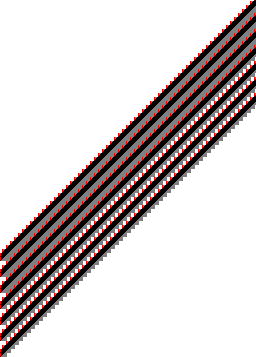
\includegraphics[width=0.4\textwidth]{st_diagrams/stencil7x7_linear.png}};
            \draw [->] (image.south west) -- ++(2,0) node[right]{\footnotesize\textit{Time}};
            \draw [->] (image.south west) -- ++(0,2) node[rotate=90, above]{\footnotesize\textit{Address}};
        \end{tikzpicture}
        \label{fig:st_stencil_naive}
    }
    \qquad
    \subfloat[The spatial temporal diagram of a 7x7 stencil with a column of size 4 ordering.]{
        \centering
        \begin{tikzpicture}
            \node (image) at (0,0) {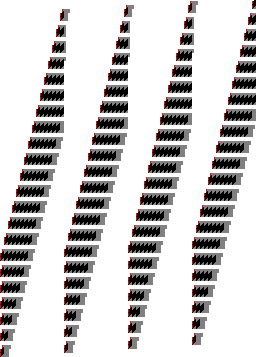
\includegraphics[width=0.4\textwidth]{st_diagrams/stencil7x7_column_4.png}};
            \draw [->] (image.south west) -- ++(2,0) node[right]{\footnotesize\textit{Time}};
            \draw [->] (image.south west) -- ++(0,2) node[rotate=90, above]{\footnotesize\textit{Address}};
        \end{tikzpicture}
        \label{fig:st_stencil_column}
    }

    \caption{
        The spatial temporal diagrams of a 7x7 stencil. The vertical axis describes the location in a 2D array which is mapped to 1D address space. The horizontal axis describes time. \fsquare{red} are addresses of cache lines that are brought into cache. \fsquare{black} are addresses being accessed. \fsquare{gray} are addresses in cache.
    }
    \label{fig:st_stencil}
\end{figure}

% fig:stencil_naive_loading_pattern
\begin{figure}[!hb]
    \centering
    
    \subfloat[Ideal cache size, only minimal amount of loading is required.]{
        \centering
        \makebox[0.4\columnwidth][c]{
            \begin{tikzpicture}[scale=0.25, decoration = {
                markings, mark = between positions 0.3cm and 0.95 step 0.25cm with {\arrow{stealth}}
            }]
                \fill[gray!50]  ( 6, 6) rectangle +(10, 1);
                \fill[gray!50]  ( 0, 2) rectangle +(16, 4);
                \fill[gray!50]  ( 0, 1) rectangle +(10, 1);
                \fill[gray!100] (10, 1) rectangle +( 1, 1);

                \draw[step=1,gray!25] (0, 0) grid (16, 8);
                \draw[black, postaction = decorate] (8.5, 4.5) -- +(5, 0);
                \draw[black, dashed] (13.5, 4.5) -- (2.5, 3.5);
                \draw[black, postaction = decorate] (2.5, 3.5) -- +(6, 0);
                \draw[red] (6,1) rectangle +(5, 5);
            \end{tikzpicture}
        }
        \label{fig:stencil_naive_loading_pattern_ideal}
    }
    \qquad
    \subfloat[Cache too small, data gets evicted before any potential reuse.]{
        \centering
        \makebox[0.4\columnwidth][c]{
            \begin{tikzpicture}[scale=0.25, decoration = {
                markings, mark = between positions 0.3cm and 0.95 step 0.25cm with {\arrow{stealth}}
            }]
                \fill[gray!50]  (10, 2) rectangle +( 6, 5);
                \fill[gray!50]  ( 0, 1) rectangle +( 8, 5);
                \fill[gray!100] ( 8, 1) rectangle +( 1, 5);

                \draw[step=1,gray!25] (0, 0) grid (16, 8);
                \draw[black, postaction = decorate] (12.5, 4.5) -- +(1, 0);
                \draw[black, dashed] (13.5, 4.5) -- (2.5, 3.5);
                \draw[black, postaction = decorate] (2.5, 3.5) -- +(4, 0);
                \draw[red] (4,1) rectangle +(5, 5);
            \end{tikzpicture}
        }
    }
    \caption{
        \TODO{write this}
    }
    \label{fig:stencil_naive_loading_pattern}
\end{figure}

The minimum amount of cachelines cached $M_l$, and therefore needed, of cache line size of $L$ elements to stay in the ideal case is correlated by the stencil size and width of the input array:

\TODO{Maths}

\begin{equation}
    M_l \geq \ceil{\frac{I_w + S_w}{L}} S_h \label{eq:stencil_naive_optimal_memory}
\end{equation}

While in most cases \TODO{examples} this enough to fully exploit L2 caches, this can be unoptimal in regard to the L1 cache.
\TODO{Example}
The amount of cache lines needed to be feteched from memory $F$ is bound by the worse case (eq. \ref{eq:stencil_naive_optimal_memory} is not satisfied) where we consistently evict data from cache before we can reuse:

\[
    F \leq \ceil{\frac{I_w + S_w}{L}} I_h S_h
\]

If equation \ref{eq:stencil_naive_optimal_memory} is satisfied, the amount of fetches $F$ is no longer depedent on the stencil height $S_h$

\[
    F = \ceil{\frac{I_w + S_w}{L}} I_h
\]

\TODO{GPU threading is different from CPU stuff yada yada}
With multiple threads active, even more data is required to be kept in cache for optimal usuage.
In the best case, all threads are cohered with overlapping accesses, and in the worst case, threads will be spread out more with less overlapping accesses.
Threads in GPUs are grouped by warps, threads contained within are always cohered, and therefore a guarantee for overlapping accesses.
Therefore, only when multiple warps are executed on the same SM, divergence in accesses can occur.
A single warp of 32 threads uses $\ceil{\frac{32 + S_w}{l}} S_h$ cache lines when the threads cover a single rows. 
When the warp is split between 2 rows, the cache needs to be slightly bigger: $\ceil{\frac{32 + 2 S_w}{l}} S_h$.

Ideally, the whole input array would fit on the cache, but a sufficiently large input (i.e. a $2048\times2048$ 32-bit floating point array uses 16 MiB) will not fit on the L2 caches of modern GPUs ($\approx6$MiB of L2 data cache, Volta V100) and cache misses are unavoidable.
Even if data would fit on the L2 cache, there would still be potential cache misses at the L1 cache (128 KiB, Volta V100).

\TODO{More figures like in fig. \ref{fig:stencil_naive_loading_pattern}, but for GPU/multithreading}

\vspace{2cm}

Using the model described in section \ref{sec:cache_gpu} can be used to estimate the cache misses of the naive implementation and the model parameters are summarized in table \ref{tab:stencil_naive_model}.
Calculating the reuse for an iteration of $s_y$, $i_x$, and $i_y$ is fairly trivial.

\TODO{These are the calculations adapted from Lam et al. 1991. I'm not really sure if I should do this. They feel not very ellegant, and more like a black box system\dots}
$s_x$ is ommited due to it only loading a singular value during one loop and has therefore no reuse.
During a single step of $s_y$ an entire row of all $S_w$ elements from the stencil has been loaded.
A single step on $i_x$ processes the output of a singular element, which means an entire stencil is read.


\begin{table}[H]
    \centering
    \begin{tabular}{|c||c|c|c|c||c|c|c|c|}
        \hline
        Array & \multicolumn{4}{c||}{Reuse} & \multicolumn{4}{c|}{Self-Interference}
        \\ \hline
        & $i_x$ & $i_y$ & $s_x$ & $s_y$
        & $i_x$ & $i_y$ & $s_x$ & $s_y$
        \\ \hline
        X & $(S_w - 1)S_h$ & $(S_h - 1) S_w I_w$ & - & $S_w$
        & &  & 0 & 0

        \\ \hhline{*{9}{=}}
        Array & \multicolumn{4}{c||}{Footprint} &  \multicolumn{4}{c|}{References}
        \\ \hline
        & $i_x$ & $i_y$ & $s_x$ & $s_y$ & \multicolumn{4}{c|}{}
        \\ \hline
        X & $S_wS_h/C$ & $I_wS_h/C$ & $1/C$ & $S_w/C$ &
        \multicolumn{4}{c|}{$I_w I_h S_w S_h$}
        \\ \hline
    \end{tabular}

    \caption{
        The reuse, self-interference, and footprint of the naive implementation of stencils during a single step of iterating on $i_x$, $i_y$, $s_x$, and $s_y$.
        \TODO{Calculate self interference}
    }
    \label{tab:stencil_naive_model}
\end{table}

\subsection{Tiling}
\label{sec:stencil_tiled}
A common used optimization is by dividing the work into works as described in \ref{sec:optimization_blocked}.
\TODO{blablablabla}

The minimum required cache for optimal tiling is depedent on \TODO{\dots} tiling size $t$

\begin{equation}
    M_l \geq \ceil{\frac{t + S_w}{L}} S_h \label{eq:stencil_tiling_memory}
\end{equation}

The largest possible tiling size $t$ is derived by inverting equation \ref{eq:stencil_tiling_memory}

\begin{equation}
    t \leq \frac{L M_l}{S_h} - S_w
\end{equation}

Since equation \ref{eq:stencil_tiling_memory} can always be satisfied by adjusting $t$, we can have a lower upper bound on the amount of cache line fetches $F$:

\begin{equation}
    F \leq \ceil{\frac{I_w}{t}} \ceil{\frac{t + S_w}{L}} \ceil{\frac{I_h}{t}} (t + S_h)
    \label{eq:stencil_tiling_fetches}
\end{equation}

\TODO{Maybe remove this. Probably just keep it, so we can plot our expected number of cache line fetches}
We can define the number cache lines fetched in terms of the available cache by substituting equation \ref{eq:stencil_tiling_memory} into equation \ref{eq:stencil_tiling_fetches}:

\begin{equation}
    F \leq \ceil{\frac{I_w}{\frac{L M_l}{S_h} - S_w}} \ceil{\frac{\frac{L M_l}{S_h} - S_w + S_w}{L}} \ceil{\frac{I_h}{\frac{L M_l}{S_h} - S_w}} \left(\frac{L M_l}{S_h} - S_w + S_h\right)
\end{equation}

\begin{equation}
    F \leq \frac{I_w I_h M_l}{(\frac{L M_l}{S_h} - S_w)^2 S_h} (\frac{L M_l}{S_h} - S_w + S_h)
\end{equation}
\TODO{simplify this further by relaxation perhaps?}


\TODO{GPU/multithreading notes}

\section{Matrix Multiplication}

\subsection{Naive}

Given the output matrix of size $I_w \times I_h$ with input matrices of size $I_w \times D$ and $D \times I_h$, we can start reusing in the naive case only if

\begin{equation}
    \label{eq:mm_naive_minimum_cache}
    M_l > \ceil{\frac{D}{L}} + D
\end{equation}

If equation \ref{eq:mm_naive_minimum_cache} is not satisfied then there is no reuse of data possible, and the amount of cache line fetches is

\begin{equation}
    F = \left( \ceil{\frac{D}{L}} + D \right) I_w I_h
\end{equation}

\TODO{Split figure \ref{fig:st_matrix} up into their parts for better flow}
% fig:st_matrix
\begin{figure}[!h]
    \centering
    \subfloat[The spatial temporal diagram of matrix multiplication with linear ordering.]{
        \begin{tikzpicture}[spy using outlines={rectangle, magnification=4,connect spies}]
            \node (image) at (0,0) {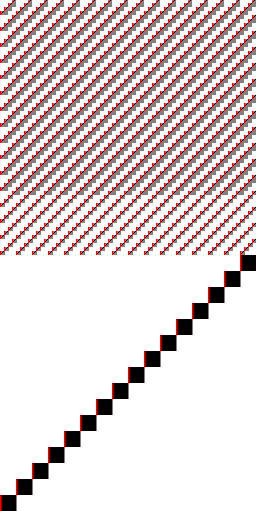
\includegraphics[width=0.25\textwidth]{st_diagrams/matrix_linear.png}};
            \draw [->] (image.south west) -- ++(2,0) node[right]{\footnotesize\textit{Time}};
            \draw [->] (image.south west) -- ++(0,8.5) node[rotate=90, above left]{\footnotesize\textit{Memory Addresses}};

            \coordinate (p) at (0, 1);
            \coordinate (v) at (3.3, 2);
            \spy[width=2.4cm,height=4cm] on (p) in node [fill=white] at (v);
        \end{tikzpicture}
        \label{fig:st_matrix_naive}
    }
    \qquad
    \subfloat[The spatial temporal diagram of a matrix multiplication with a column of size 4 ordering.]{
        \centering
        \begin{tikzpicture}[spy using outlines={rectangle, magnification=4,connect spies}]
            \node (image) at (0,0) {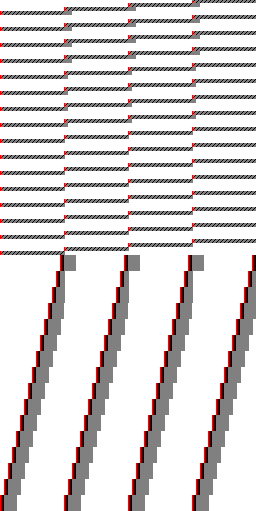
\includegraphics[width=0.25\textwidth]{st_diagrams/matrix_column_4.png}};
            \draw [->] (image.south west) -- ++(2,0) node[right]{\footnotesize\textit{Time}};
            \draw [->] (image.south west) -- ++(0,8.5) node[rotate=90, above left]{\footnotesize\textit{Memory Addresses}};

            \coordinate (p) at (0, 1);
            \coordinate (v) at (3.3, 2);
            \spy[width=2.4cm,height=4cm] on (p) in node [fill=white] at (v);
        \end{tikzpicture}
        \label{fig:st_matrix_column}
    }

    \caption{
        The spatial temporal diagrams of a matrix multiplication. The vertical axis describes the location in a 2D array which is mapped to 1D address space. The horizontal axis describes time. \fsquare{red} are addresses of cache lines that are brought into cache. \fsquare{black} are addresses being accessed. \fsquare{gray} are addresses in cache.
    }
    \label{fig:st_matrix}
\end{figure}

\subsection{Tiling}
